%summary for IMA

\documentclass[french]{article}
\usepackage[utf8]{inputenc}
\usepackage[T1]{fontenc}
\usepackage{babel}
\usepackage{lmodern}
\usepackage{graphicx}
\usepackage{tikz}
\usetikzlibrary{arrows}

\usepackage{amsmath}
\usepackage{amsfonts}

\usepackage{float}

\title{Ima}
\date{}
\author{L3 RI}


\begin{document}
\maketitle
\tableofcontents
\newpage

\section{Introduction}
On considère des images en niveaux de gris. À chaque pixel d'une image
on associe donc une valeur dans ${0\dots255}$
\subsection{Histogramme}
L'histogramme d'une image donne des informations que la densité de
chaque valeur.
\paragraph{Définition} L'histogramme d'une image $I$ est une fonction
discrète qui associe à chaque valeur d’intensité le nombre de pixels
prenant cette valeur.
$$
\begin{array}{rccl}
h_t : & {0\dots255} & \to & \mathbb{N} \\
 & n & \mapsto & \text{Card}\left\{(x,y) | I(x,y) = n\right\}\\
\end{array}
$$
\subparagraph{Remarque} Si on a une image de taille $p\times q$ alors
$\sum_{n = 0}^{255} = p*q$

\subparagraph{Propriété} L'histogramme d'une image et de sa translation
sont les mêmes. Ce n'est donc \emph{pas une caractéristique de l'image}.

\paragraph{Interprétation} Si l'histogramme est condensé sur les valeurs
faibles (resp. sur les fortes) alors l'image est \emph{sous-exposé} (resp.
\emph{surexposé}).

\paragraph{Égalisation} On peut normaliser un histogramme condensé en
étalant ces valeurs sur toute la plage $[|0, 255|]$. Cela améliore le
contraste.

Si l'image occupe déjà toute la plage on utilise un autre algorithme basé
sur l'histograme cumulé:
$$
\begin{array}{rccl}
h_c : & {0\dots255} & \to & \mathbb{N} \\
 & n & \mapsto & \text{Card}\left\{(x,y) | I(x,y) < n\right\}\\
\end{array}
$$

On répartit pour obtenir un histogramme linéaire.

\begin{figure}[h]
\begin{center}
{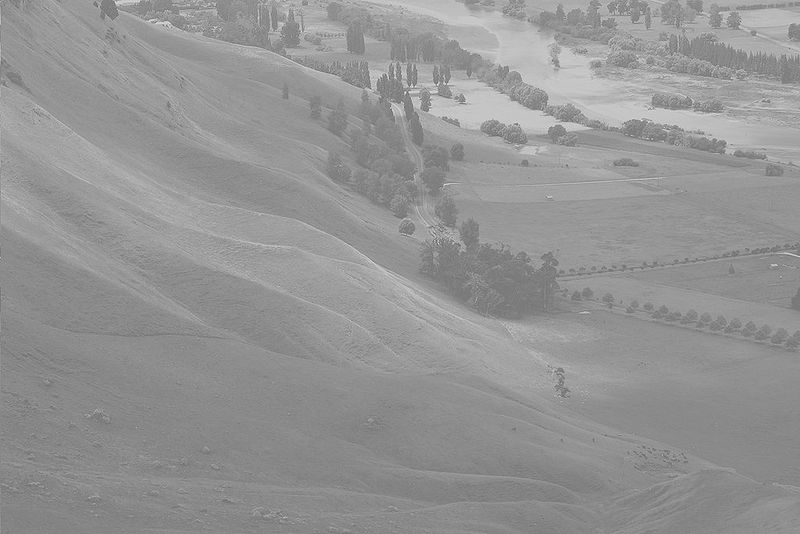
\includegraphics[scale=0.16]{images/histo01.jpg}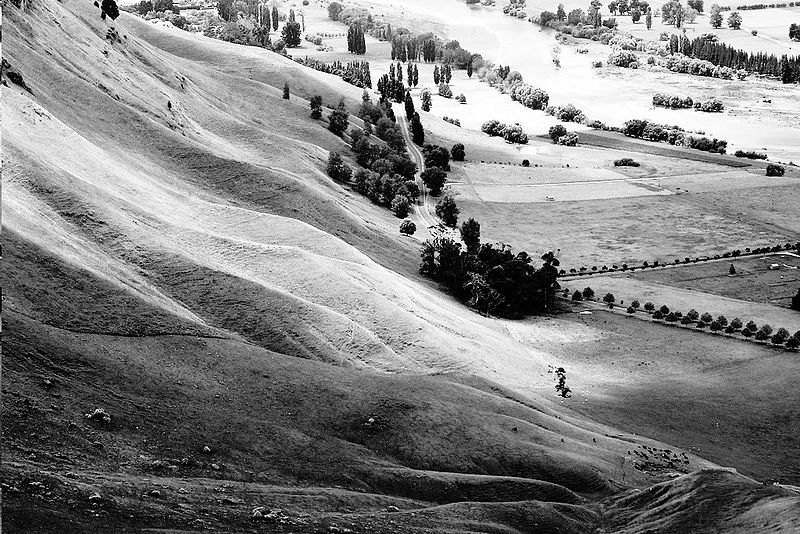
\includegraphics[scale=0.16]{images/histo03.jpg}} 
\end{center}
\begin{center}
{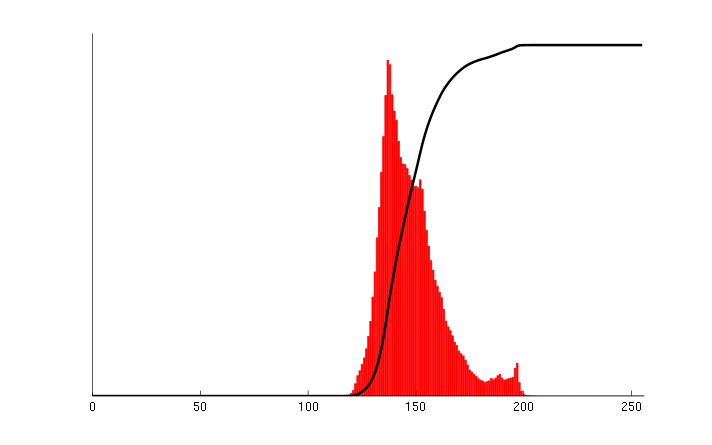
\includegraphics[scale=0.16]{images/histo02.png}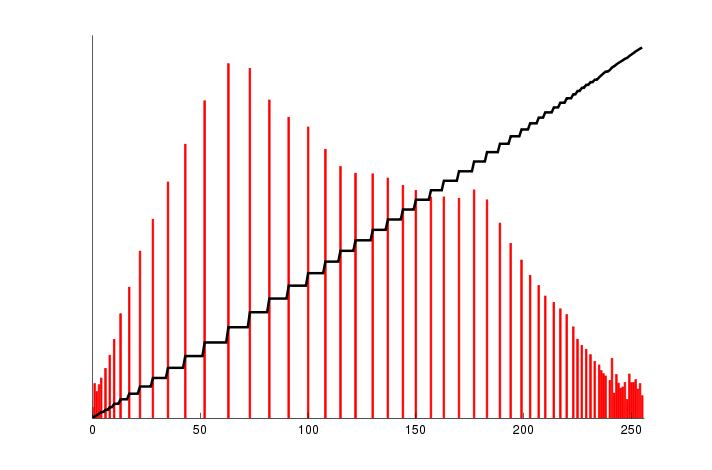
\includegraphics[scale=0.16]{images/histo04.png}} 
\end{center}
\caption{Résultat de l'Algorithme d'égalisation de l'histogramme}
(Source : Wikipédia)
\end{figure}

\subsection{Transformations géométriques}
Le résultat d'une transformation géométrique (rotation, transformations
affines, etc.) aboutit généralement à ce que les pixels de l'image
d'origine n'aient plus des coordonnées entières.

\paragraph{Inteprolation d'intensité} L'interpolation permet de déduire
la couleur des positions entières à partir des positions non entières
connues.

Exemple : Plus proches voisins, bilinéaire, bicubique, par convolution.

\paragraph{Convolution 1D}
$$(f * g)(x) = \int_{-\infty}^{+\infty}f(x-t) g(t) dt$$

\paragraph{Convolution 2D}
Soit $g$ une fonction telle que $\int_{\Bbb{R}^2}g(x,y)dxdy=1$.
On définit l'image traitée par convolution:
$$I_{\text{convol}} = I(x,y) * g(x, y) = \int_{\Omega}g(x - a, y -b) I(a,b) da db$$

L'influence des voisins sur le résultat en une position donnée va donc
dépendre du noyau de convolution $g$ utilisé. Cela permet de lisser mais
peut aussi induire du flou.

Ex : Noyau moyenneur, gaussienne, floude bougé, etc.

\subparagraph{Remarque} Pour débruiter, un filtre médian est plus
efficace qu'un filtre moyenneur.

\section{Dérivées, opérateurs, discrétisation}
\subsection{Dérivées partielles}
\subsection{Opérateurs usuels}
\subsection{Équation aux dérivées partielles}
\subsection{Discrétisation}
\subsection{Stabilité d'un schéma numérique}

\section{Restauration d'images}
\subsection{Régularisation}
\subsection{Minimisation de fonctionnelle}
\subsection{Débruitage}
\subsection{Défloutage}
\subsection{Inpainting}

\section{Segmentation}
\subsection{Seuillage d'histogramme}
\subsection{Algo K-means}
\subsection{Limites algos globaux}
\subsection{Region growing}
\subsection{Split and merge}
\subsection{Méthode markovienne}
\subsection{Graph-Cuts}
\subsection{Détecteur de Canny}
\subsection{Segmentation par contours actifs}

\section{Transformée de Fourier}
\subsection{Transformée 1D}
\subsection{Transformée 2D et 2D discrète}
\subsection{Transformée sur des images}

\end{document} 

